\documentclass[12pt]{article}

% Packages
\usepackage[utf8]{inputenc}
\usepackage{amsmath, amssymb, amsthm}
\usepackage{geometry}
\usepackage{graphicx}
\usepackage{hyperref}
\usepackage{parskip}
\usepackage{mathrsfs}
\usepackage[most]{tcolorbox}
\tcbuselibrary{breakable}
\tcbset{
    parbox=false,
    breakable
}
\usepackage{algorithm}
\usepackage{algpseudocode}
\usepackage{enumitem}
\usepackage{cancel}
\usepackage{witharrows}
\usepackage{minted}
\usepackage{array}
\usepackage{booktabs}

% Custom commands
\newtcolorbox{altbox}[1][]{
   	enhanced,
		title = Example,
		attach boxed title to top left = {
				xshift = 1em,
				yshift*=-\tcboxedtitleheight/2
			},
    #1 % Allows for extra local overrides
}

\newtheoremstyle{spaced}
    {\parskip}   % Space above
    {\parskip}   % Space below
    {\itshape}   % Body font
    {}           % Indent
    {\bfseries}  % Head font
    {.}          % Punctuation
    {.5em}       % Space after head
    {}

\theoremstyle{spaced}
\newtheorem{lemma}{Lemma}
\theoremstyle{spaced}
\newtheorem{definition}{Definition}

\newcounter{N}
\newcommand{\num}{
    \vspace{2em}
    \boxed{\refstepcounter{N}\theN}
    \ignorespaces
}
% Page setup
\geometry{a4paper, margin=1in}

% Title
\title{PARALLEL COMPUTING exam questions PT1}
\author{Claudio Tessa}
\date{\today}

\begin{document}

\maketitle

\tableofcontents
\newpage

\section{Part 1}
\input{sections/exercise1-1.tex}
\input{sections/exercise1-2.tex}
\input{sections/exercise1-3.tex}
\input{sections/exercise1-4.tex}

\section{Part 2}
\subsection{Exercises 2-1}

\num Please describe how the Pack parallel pattern works. How is it implemented (pseudo code and PRAM complexity required)?

\begin{tcolorbox}
	Used to eliminate unused elements from a collection:

	\begin{enumerate}
		\item Convert input array of Booleans into integer 0s and 1s;
		\item Perform an exclusive scan of this array with the SUM operation;
		\item Write values in the output array based on the offset
	\end{enumerate}



	\begin{minted}{cpp}
        if(InitialMask[i])
            out[ExScanOf1[i]] = input[i];     
    \end{minted}

	If executed on $N$ execution units, step 1 and 2 have a complexity of $O(1)$, while step 2 has a time complexity of $O(\log N)$, therefore the total time complexity is $O(\log N)$. Work is $O(N)$.
\end{tcolorbox}

\num Consider the following nested loop:

\begin{minted}{text}
    for (j = 0; j < 999; j++) {
        for (i = 2; i < 999; i++) {
            a[i][j] = f(a[i-2][j]);
        }
    }
\end{minted}

Evaluate the cache-friendliness of this code and consider its relationship to parallelizability. How does the memory layout of the array affect performance, and what changes could improve cache utilization vs parallelizability? Justify your answer. Assume that \texttt{a} stores integers.

\begin{tcolorbox}
	Original code is fully parallelizable with respect to loop \texttt{j} if function \texttt{f} is \textbf{safe} and it is partially parallelizable with respect to loop \texttt{i}.

	The original code is poor with respect to cache friendliness because the variable \texttt{a} is accessed column-wise. Swapping the two loops fixes cache friendliness. Tiling could be another approach to improve cache friendliness and parallel computation
\end{tcolorbox}

\num How and under what conditions can the following code be parallelized? Is there a way to write the code for better parallelization? Assume that a and b store integers.

\begin{minted}[autogobble]{text}
    for (i=4; i<100; i++) {
        for (j=1; j<100; j++)
            a[i][0] *= f(a[i][j]);
        for (j=0; j<100; j++)
            b[i-4][j] += f(b[i][j]);
    }
\end{minted}

\begin{tcolorbox}
	Assuming that \texttt{f} is a safe function:
	\begin{itemize}
		\item The \texttt{a} loop (first inner loop): each row \texttt{i} is independent from each other $\implies$ fully parallelizable.
		\item The \texttt{b} loop (second inner loop): there is a loop carried dependency $\implies$ we can only parallelize with respect to loop \texttt{j} but not with respect to loop \texttt{i}.
	\end{itemize}
	To make parallelization better, we can remove the loop-carried dependency, using a temporary copy of \texttt{b}, example:
	\texttt{copy\_b = b} before the loop, and then in the \texttt{b} loop:
	\texttt{b[i - 4][j] += f(copy\_b[i][j]);}
\end{tcolorbox}

\num Which loop can be parallelized and under which conditions? Does the overhead of the runtime have an impact on the parallelization of the loops? When and on which target architecture?

\begin{minted}[autogobble]{text}
    for (j=1; j<1000; j++)
        for (i=0; i<10; i++)
            a[i][j] = f(a[i][j]);
\end{minted}

\begin{tcolorbox}
	\textbf{Both} loops can be parallelized because there are no loop-carried dependencies between iterations (assuming \texttt{f} is a safe function).

	However, for performance, you should parallelize the outer loop (\texttt{j}). The overhead of the runtime is critical here: the inner loop has a count of only 10, which is too small to justify the cost of thread creation and management.

	This is worse on CPUs (where spawning threads causes a greater slowdown) than GPUs, as GPUs have explicit hardware that manages thread creation. But a block size of 10 on a GPU, would be a significant waste of resources (as warp size is typically of 32 threads).
\end{tcolorbox}

\num Please describe the parallel gather pattern, including assumptions, complexity, and examples.

\begin{tcolorbox}
	Given a collection of ordered indices, read data from the source collection at each index, and write data to the output collection in index order. It can be seen as the inverse of scatter.

	Typically assumes a CREW PRAM (Concurrent Read, Exclusive Write) model to allow multiple threads to read from the same source location simultaneously.

	Time complexity is $O(1)$ since all reads happen in parallel. Work is $O(N)$, one operation per element.

	An \textbf{example} is rotating an image: the new target pixel need to \textit{gather} the color from the source pixel.
\end{tcolorbox}

\num Please describe how the Split parallel pattern works. How is it implemented (pseudo code required)?

\begin{tcolorbox}
	Split rearranges data so that all elements of the input are moved to either the lower or upper part of the output collection, given on a boolean collection that tells in which of the two portions an element will go. Relative ordering withing the lower/upper half is kept.

	\begin{minted}[autogobble]{cpp}
        LastOf0 = ExScanOf1[last] + 1;
        if(InitialMask[i])
            out[ExScanOf1[i] + LastOf0] = DataInput[i];
        else
            out[ExScanOf0[i]] = DataInput[i];
    \end{minted}
\end{tcolorbox}

\num Please describe how the Unzip parallel pattern works. How is it implemented (pseudo code and PRAM complexity required)?

\begin{tcolorbox}
	Unzip is the reverse of zip. Given a sequence, separates them into subarrays at certain offset. For each thread, the pseudocode un:

	\begin{minted}[autogobble]{cpp}
        X[i] = A[2 * i]; // even index
        Y[i] = A[2 * i + 1]; // odd index
    \end{minted}

	\textbf{PRAM complexity} assuming CREW:
	\begin{itemize}
		\item \textbf{time} complexity: $O(1)$ since all operations happen simultaneously
		\item \textbf{work} complexity $O(n)$, 2 operations per thread
	\end{itemize}
\end{tcolorbox}

\num Please describe how the parallel zip pattern works, its complexity, and how it could be parallelly implemented.

\begin{tcolorbox}
	The Zip pattern combines two input arrays into a single output array, interleaving the input elements. In the PRAM model (assuming N processors), it achieves O(1) step complexity and O(N) work complexity because every pairing operation is completely independent.

	It is parallelly implemented as a straightforward map operation: the system launches $N$ threads, where each thread $i$ simultaneously reads the $i$-th elements from both source arrays and writes the first input element to the output array at index $2i$ and the second input element at index $2i + 1$, requiring zero synchronization.
\end{tcolorbox}

\num Can you remove a flow dependency? Yes/No, and in case, how?

\begin{tcolorbox}
	\textbf{No}, you can generally not remove flow dependencies (Read-After-Write) because they are \textit{true} dependencies.

	Unlike anti- or output dependencies, which can be eliminated by register renaming, flow dependencies are a hard ordering constraint required for correctness. The only way to remove it is to fundamentally \textbf{alter the algorithm} (e.g., restructuring the calculation chain).
\end{tcolorbox}

\num Please describe what \textbf{relaxing} the sequential consistency memory model means and why it is done.

\begin{tcolorbox}
	\textbf{Relaxing} the sequential consistency memory model means abandoning the strict guarantee that every thread sees all memory operations in the exact order specified by the program code. Instead, the hardware (CPU) and the compiler are permitted to reorder memory instructions, meaning that different threads may perceive memory updates happening in different sequences.

	This is done for \text{performance}: strict consistency forces the processor to stall and wait for every single memory access to propagate to main memory.
\end{tcolorbox}

\num Please describe how the “Permutation collision resolution” works. Is it related to the parallel gather pattern?

\begin{tcolorbox}
	No. The permutation collision resolution is related to the scatter pattern. A collision occur when, in the scatter pattern, two input locations map to the same output location. The permutation collision resolution simply states that collisions are illegal (check for collisions in advance). Therefore, if there are no collisions, the output is simply a permutation of the input.
\end{tcolorbox}

\num Please describe how DOALL loops could be parallelized using a known parallel pattern.

\begin{tcolorbox}
	DOALL loops are parallelized using the \textbf{Map} pattern. Because a DOALL loop implies that every iteration is completely independent of the others (no loop-carried dependencies), the problem can be treated as applying a function $f(x)$ to every element of the input collection simultaneously.

	The total index range (0 to N) is partitioned into chunks, and these chunks are distributed across parallel threads (using either static or dynamic scheduling) so that each thread executes the loop body for its assigned indices concurrently.
\end{tcolorbox}

\num Please describe how the shift parallel pattern could be implemented in a parallel way.

\begin{tcolorbox}
	The shift pattern is implemented as a Map operation where each thread reads an input element at a fixed offset (e.g., \texttt{input[i + offset]}) and writes it to its current position output[i].

	To implement it, the standard approach is Tiling with Shared Memory. A thread block cooperatively loads a segment of data (plus the boundary elements corresponding to the shift size) into the fast shared memory. After a barrier synchronization, threads read the shifted values from shared memory and write the result to global memory.

	This prevents unaligned memory accesses (non-coalesced reads) that would occur if threads tried to read directly from global memory with an arbitrary offset.
\end{tcolorbox}

\num Please define parallel pattern reduce: assumptions, complexity, and example.

\begin{tcolorbox}
	The Reduce pattern combines a collection of elements into a single summary value by repeatedly applying a specific operator. The assumption is that the operator must be \textbf{associative}. For example: sum all the elements of the array.

	A parallel reduction uses a tree-based approach that performs \textbf{total work} $O(N)$ and time complexity $O(\log N)$ (the tree is deep $\log N$).
\end{tcolorbox}

\num Please describe how the Unpack pattern could be implemented.

\begin{tcolorbox}
	The Unpack pattern is implemented by combining the Scan and Map:
	\begin{itemize}
		\item First, an exclusive Scan (prefix sum) is performed on the boolean mask;
		\item Then, a Map is executed over the destination array: if the mask at index \texttt i is true, the thread reads the input value using the index calculated by the scan and writes it to output \texttt i; otherwise, it fills the slot with a default identity value (like 0).
	\end{itemize}
\end{tcolorbox}

\num Please define what a parallel pattern scan is: assumptions, complexity, and example.

\begin{tcolorbox}
	The Scan pattern computes all partial reductions of a sequence, transforming an input $[a_0, a_1, \dots, a_n]$ into an output where each element $y_i$ is the combination of all preceding inputs up to that point.

	The main assumption is that the operator must be \textbf{associative} (e.g., addition), which allows the algorithm to reorder calculations into a tree structure.

	In terms of complexity, a work-efficient scan performs $O(N)$ work (matching the sequential baseline) but achieves a critical path of $O(\log N)$.

	An example is prefix sum.
\end{tcolorbox}

\num Describe how the scope of variables can be specified upon entering an OpenMP parallel region.

\begin{tcolorbox}
	\texttt{\#pragma omp parallel shared(a) private(b)}
	\begin{itemize}
		\item \texttt{shared(...)}: all threads access the single original memory location;
		\item \texttt{private(...)}: each thread creates its own \textit{uninitialized} local copy of the variable;
		\item \texttt{firstprivate(...)}: similar to \texttt{private}, but the local copy is \textit{initialized} with the value that the variable had vefore entering the parallel region;
		\item \texttt{default(mode)}: set the default mode for all variables not listed (e.g., \texttt{default(shared)}.
	\end{itemize}
\end{tcolorbox}

\subsection{Exercises 2-2}

\num What is the impact of memory coalescing on DRAM access efficiency in CUDA?

\begin{tcolorbox}
	When all threads of a warp execute a load instruction, if all accessed locations fall into the same burst section (coalesced access), only one DRAM request will be made and the access is fully coalesced.
\end{tcolorbox}

\num What is the purpose of using shared memory in tiled matrix multiplication? Is the corner turning technique relevant for this purpose?

\begin{tcolorbox}
	Reading A and B in a matrix multiplication results in A read in non-coalesced way and B read in a coalesced way. To improve performance, we copy the data into shared memory, allowing both input matrices to be accessed coalesced in both cases (corner turning).
\end{tcolorbox}

\num Please describe how priority scatter works.

\begin{tcolorbox}
	Given a collection of input data, and a collection of location, \textbf{scatter} copies the input data in the output data, at the location specified by the locations collection.

	The location array could map two or more input elements to the same location. In this case, priority scatter solves this write conflict by allowing only the processor with highest priority to write.
\end{tcolorbox}

\num How can a CUDA programmer judge if an access is coalesced?

\begin{tcolorbox}
	By checking if consecutive threads in a warp are accessing consecutive memory addresses. Mathematically, the access is coalesced if the memory accesses are in the form of \texttt{Mem[Base + ThreadIdx.x]}. This creates a sequential pattern that allows the memory controller to merge the individual requests into a single transaction.

	If the threads access memory e.g. randomly, the hardware must split the operation into multiple separate transactions, signaling uncoalesced access.
\end{tcolorbox}

\num Describe the corner turning technique. How the size of the shared memory is defined in this technique?

\begin{tcolorbox}
	\textit{See corner turning technique definition in a previous question}

	The allocated size is primarily defined by the tile dimensions (e.g., $TILE\_WIDTH \times TILE\_WIDTH$). However, in \textbf{Corner Turning}, the size is frequently defined as
	$$
		TILE\_WIDTH \times (TILE\_WIDTH + 1)
	$$
	This extra column of padding shifts the data layout in shared memory to ensure that when threads read down a column, they access different memory banks, preventing Bank Conflicts.
\end{tcolorbox}

\num Does it make sense to use the corner-turning optimization in a non-GPU-based architecture? Why?

\begin{tcolorbox}
	\textbf{Yes}. The corner-turning technique is effective also on CPUs to maximize spatial locality in the cache. CPUs fetch memory in cache lines; if a program accesses data column-wise in a row-major array, it loads an entire cache line but uses only a single value, wasting bandwidth and causing cache pollution.

	Corner turning reorganizes the data so that the CPU reads contiguous memory addresses, enabling the use of SIMD instructions, which require aligned data for maximum performance.
\end{tcolorbox}

\num Please briefly describe the differences between Memory coherence and memory consistency.

\begin{tcolorbox}
	\begin{itemize}
		\item Memory \textbf{coherence} ensures that \textbf{all processors see the most recent update} to that specific location (everyone agrees that a specific variable has a specific value).
		\item Memory \textbf{consistency} defines the rules for the \textbf{ordering of operations} across multiple distinct memory addresses, ensureing the timeline of events makes sense across the entire program.
	\end{itemize}
\end{tcolorbox}

\num Please describe how merge scatter works.

\begin{tcolorbox}
	The scatter pattern, given a collection of input data and a collection of write locations, writes the data to the output collection at the indices specified by the location array.

	\textbf{Merge} is used to handle collisions when multiple input elements attempt to write to the same output location. It combines the conflicting writes using an operator (e.g., addition: the final value is the sum of the conflicting input values). This operator must be \textbf{associative} and \textbf{commutative}.
\end{tcolorbox}

\num Is DRAM burst affecting the corner-turning optimization?

\begin{tcolorbox}
	\textbf{Yes}. DRAM burst necessitates corner-turning optimization, because DRAM transfers data in fixed-size chunks (bursts), typically filling a cache line in one transaction. Accessing memory in a strided pattern like reading column-wise, pulls in a full burst but consumes only a single useful value, wasting the rest of the available bandwidth.

	Corner-turning reorganizes the data into a contiguous layout, ensuring that when a DRAM burst is fetched, every byte within it is utilized by the processor, maximizing memory throughput.
\end{tcolorbox}

\num Please briefly describe what DRAM Banking is meant for. How can CUDA take advantage of DRAM banking?


\begin{tcolorbox}
	DRAM banking partitions physical memory into independent sub-arrays (banks) that can operate in parallel, allowing the memory controller to issue a command to another bank while one is busy (e.g., activating a row).

	CUDA takes advantage of this because when a warp performs a coalesced memory access (reading contiguous data), the requests are naturally distributed across multiple active banks, preventing serialization (bank conflicts) and saturating the global memory bus.
\end{tcolorbox}

\num Describe briefly the shared memory programming model with threads and two of its implementations.

\begin{tcolorbox}
	The \textbf{shared memory} programming model involves multiple concurrent threads operating within a single unified address space, where they communicate implicitly by reading/writing to the same variables. This model relieson synchronization primitives (like locks or atomic operations) to prevent race conditions.

	Two key implementations are
	\begin{itemize}
		\item POSIX Threads (Pthreads): low-level, explicit API standard used in C/C++ that gives developers fine-grained control over thread lifecycle and synchronization;
		\item OpenMP: high-level standard that automates thread creation and work distribution via compiler pragmas (e.g., \texttt{\#pragma omp parallel})
	\end{itemize}
\end{tcolorbox}

\num Describe in detail the effect of the following OpenMP pragma.

\begin{minted}[autogobble]{text}
    #pragma omp parallel for shared(tmp) private(i, j) if (!embedded)
\end{minted}

\begin{tcolorbox}
	Parallelized the immediately following \texttt{for} loop:

	\begin{enumerate}
		\item \texttt{\#pragma omp parallel for}: creates a team of threads and divides the iterations of the following \texttt{for} loop amond those threads. At the end of the loop, there is an implicit \textbf{barrier} where all threads wait for each other to finish before the master thread resumes execution.
		\item \texttt{shared(tmp)}: means that the variable \texttt{tmp} exists in a single memory location shared by all threads.
		\item \texttt{private(i, j)}: means that each thread creates its own local instance of variables \texttt{i} and \texttt{j}. \texttt{i} is implicitly handled by OpenMP, but \texttt{j} is \textbf{uninitialized}.
		\item \texttt{if (!embedded)}: determines at runtime whether to execute in parallel or sequentially, based on the value of the \texttt{embedded} boolean variable.
	\end{enumerate}
\end{tcolorbox}

\num Which OpenMP pragma allows offloading part of the computation to an accelerator? Which clause is used to manage data transfers?

\begin{tcolorbox}
	\begin{itemize}
		\item \texttt{\#pragma omp target} is used to offload a code region to an accelerator (e.g., GPU).
		\item To manage the data transfer between the host and the device, we use the \texttt{map} clause.
	\end{itemize}
\end{tcolorbox}

\num List the factors that determine the number of threads in an OpenMP parallel region.

\begin{tcolorbox}
	The factors listed in order from highest precedence to lowest:
	\begin{itemize}
		\item \texttt{num\_threads} clause in a pragma declaration;
		\item \texttt{omp\_set\_num\_threads()} function can be called by the program before the parallel region;
		\item \texttt{OMP\_NUM\_THREADS} environment variable set by the user in the OS shell before running the program;
		\item \textbf{system default} if none of the above are set.
	\end{itemize}
\end{tcolorbox}

\num Which errors will arise compiling the following code snippet?

\begin{minted}[autogobble]{text}
    #pragma omp parallel for shared(num_steps) reduction(+:sum) default(none)
    for (i=1;i<= num_steps; i++)
    {
        x = array[i] * 2;
        sum = sum + x;
    }
\end{minted}

\begin{tcolorbox}
	The compiler will issue error regarding the \textbf{scope of the data}. The clause \texttt{default(none)} enforces that every variable inside the parallel region must be explicitly categorized (e.g., \texttt{shared}, \texttt{private}), but \texttt{x} and \texttt{array} are missing from the directives.

	Note: \texttt{i} is implicitly private in a \texttt{parallel for} loop.
\end{tcolorbox}

\num Describe the way in which 15 iterations are divided among 10 threads with a static schedule and a chunk size of 2, and with a dynamic schedule with a chunk size of 1.

\begin{tcolorbox}
	\begin{itemize}
		\item \textbf{static schedule}: the iterations are divided into fixed blocks of 2 and assigned to threads in a \textbf{round robin} fashion: thread 0 gets iterations \texttt{0, 1}, thread 1 gets \texttt{2, 3}, etc. Note how threads 8 and 9 receive no work.
		\item \textbf{dynamic schedule}: the iterations are put in a queue and threads request 1 iteration at a time. Initially, all 10 threads (0–9) will likely pick up one iteration each. The remaining 5 iterations will be assigned one by one to whichever threads finish their first task fastest.
	\end{itemize}
\end{tcolorbox}

\num It is always necessary to place an explicit barrier at the end of an OpenMP work sharing construct. Is this statement true or false? Explain.

\begin{tcolorbox}
	\textbf{FALSE}. This statement is False.

	By default, OpenMP automatically inserts an implicit barrier at the end of most work-sharing constructs (like \texttt{for}, \texttt{sections}, etc) to ensure all threads finish their assigned tasks before proceeding.
\end{tcolorbox}

\num Describe what is the effect of the following OpenMP directive:

\begin{minted}[autogobble]{text}
    #pragma omp for simd schedule(simd:static, 3)
\end{minted}

\begin{tcolorbox}
	It splits the loop iterations among the available threads (the \texttt{for} part) and simultaneously instructs the compiler to execute the iterations within each thread using SIMD vector instructions (the \texttt{simd} part).

	The clause \texttt{schedule(simd:static, 3)} dictates that the iterations are divided into chunks of exactly 3, which are assigned to threads in a \textbf{static round-robin} fashion (e.g., Thread 0 gets iterations 0-2, Thread 1 gets 3-5, etc.). The \texttt{simd} modifier in the schedule ensures the chunk boundaries are handled consistently with SIMD alignment.
\end{tcolorbox}

\subsection{Exercises 2-3}

\num Efficient parallel programming with CUDA requires knowledge about GPU architecture. Discuss this claim by providing concrete examples.

\begin{tcolorbox}
	Yes because performance gains depend on aligning code with physical hardware constraints rather than just logical correctness.

	For example, a developer must understand the SIMT (Single Instruction, Multiple Threads) execution model to avoid warp divergence, where conditional branches (\texttt{if-else}) force the hardware to serialize execution paths, leaving ALUs idle.

	Additionally, maximizing memory throughput requires knowledge of memory coalescing, structuring data access so that threads read contiguous addresses, allowing the memory controller to merge individual requests into a single transaction.
\end{tcolorbox}

\num What is Unified Memory in CUDA? When is it used?

\begin{tcolorbox}
	Unified Memory is an abstraction that lets the programmer treat the host and device memories as a single address space. Data transfers between host and device happen at runtime. It is used to simplify the programming (so that data does not need to be moved explicitly between host and device) and it might be useful for sparse/irregular workloads or in multi-GPU systems.
\end{tcolorbox}

\num Given the following CUDA kernel, discuss the impact of control divergence for different \texttt{N} values.

\begin{minted}[escapeinside=||, autogobble]{text}
    __global__ void myKernel(int *data, int N) {
        int idx = threadIdx.x + blockIdx.x * blockDim.x;
        if (idx < N) {
            if (idx |\%| 2 == 0) {
                data[idx] *= 2;
            } else {
                data[idx] += 1;
            }
        }
    }
\end{minted}

\begin{tcolorbox}
	The impact of control divergence in this kernel is severe regardless of \texttt{N}. Since CUDA threads are grouped into warps of 32 consecutive indices, the condition \texttt{idx \% 2 == 0} creates an alternating pattern. Consequently, the GPU hardware must serialize the execution, halving the throughput for the entire kernel execution.

	The value of \texttt{N} only affects the boundary check (\texttt{idx < N}). Ideally, \texttt{N} should be greater than the warp size, but the divergence explained above dominates the performance penalty.
\end{tcolorbox}

\num Is an execution configuration of <<<120, 120>>> suitable for a GPU with 40 streaming processors and 32-thread warps?

\begin{tcolorbox}
	<<<120, 120>>> means a kernel launch with 120 blocks, each with 120 threads.

	While this will execute correctly, it is \textbf{not optimal} for 32-thread warps, because 120 is not a multiple of 32, so the hardware must allocate 4 warps ($32 \times 4 = 128$) for every block, leaving 8 threads idle in every block.
\end{tcolorbox}

\num Considering the execution configuration of the previous question, how many copies of a shared variable will exist during the execution of the kernel?

\begin{tcolorbox}
	here will be exactly \textbf{120 copies} of the shared variable. In CUDA, a variable declared as shared has a scope limited to a single Thread Block. Since the execution configuration <<<120, 120>>> launches 120 distinct blocks, the GPU allocates a separate instance of that shared memory variable for each block.
\end{tcolorbox}

\num What is on-demand migration and why is it harmful for performance?

\begin{tcolorbox}
	\textbf{On-demand migration} is the automatic movement of memory pages between the host (CPU) and device (GPU) memory, triggered by a page fault when a processor attempts to access data that resides physically on the other device.

	It is harmful to performance because the fault halts execution, forcing the system to transfer data (slow) between devices before resuming.
\end{tcolorbox}

\num Control divergence only happens when the kernel contains \texttt{if-else} blocks. Is this statement true or false? Explain.

\begin{tcolorbox}
	\textbf{FALSE}.

	Control divergence occurs whenever threads within the same warp are required to execute different instructions at the same time. \texttt{if-else} blocks are the most common cause, but divergence also happens in loops where the loop condition depends for example on the thread ID.
	In this cases, the hardware must serialize the execution.
\end{tcolorbox}

\num Consider the following CUDA code fragment.

\begin{minted}[autogobble]{text}
    unsigned int t = threadIdx.x;
    unsigned int start = 2*blockIdx.x*blockDim.x;
    partialSum[t] = input[start + t];
    partialSum[blockDim.x+t] = input[start+ blockDim.x+t];

    for (unsigned int stride = 1; stride <= blockDim.x; stride *= 2)
    {
        __syncthreads();
        if (t % stride == 0) { partialSum[2*t]+= partialSum[2*t+stride]; }
    }
\end{minted}

If the block size is 1024 and the warp size is 32, how many warps in a block will have divergence during the iteration where the stride is equal to 64?

\begin{tcolorbox}
	\textbf{16}.

	With a block size of 1024 and a warp size of 32, there are $1024 / 32 = 32$ total warps in the block (indexed 0 to 31). The condition \texttt{if (t \% 64 == 0)} is true only for threads that are multiples of 64 (i.e., threads 0, 64, 128, ..., 960). These active threads correspond to the first thread of every even-numbered warp (e.g., thread 64 is the first thread of Warp 2).

	\begin{itemize}
		\item \textbf{Even} Warps (0, 2, ... 30) contain 1 active thread and 31 inactive threads. Since threads in the same warp must take different paths, \textbf{these 16 warps diverge}.
		\item \textbf{Odd} Warps (1, 3, ... 31): Contain 0 active threads (e.g., Warp 1 covers threads 32–63, none of which are multiples of 64). These warps are uniformly inactive and do not diverge.
	\end{itemize}

\end{tcolorbox}

\num Assume that each CUDA atomic operation takes 4ns to complete in L2 cache and 100ns to complete in DRAM. If 90\% of atomic operations in a program hit in L2 cache, what is the approximate throughput for atomic operations on the same global memory variable?

\begin{tcolorbox}
	To estimate the throughput, we first calculate the Average Memory Access Time (AMAT) for a single atomic operation.
	$$
		\text{AMAT} = (0.9 \times 4 \text{ ns}) + (0.1 \times 100 \text{ ns}) = 13.6 \text{ ns}
	$$
	The throughput is the inverse of this average latency:
	$$
		\text{Throughput} = \frac{1}{13.6 \times 10^{-1} \text{ s}} \approx 73.5 \times 10^6 \text{ operations/second}
	$$
\end{tcolorbox}

\num Is it possible to launch multiple different CUDA kernels in parallel? How?

\begin{tcolorbox}
	\textbf{Yes}. This is achieved using \textbf{CUDA Streams}. By default, operations in the main stream (Stream 0) execute sequentially, but if you create separate non-default streams (using \texttt{cudaStreamCreate}) and launch different kernels into them (e.g., \texttt{kernelA<<<..., stream1>>>} and \texttt{kernelB<<<..., stream2>>>)}, the GPU hardware scheduler can execute them in parallel.

	This overlap is possible only if there are sufficient hardware resources (Streaming Multiprocessors) available to accommodate the blocks from both kernels and no synchronization barriers exist between the streams
\end{tcolorbox}

\num What is “false sharing”? Write an example of an OpenMP program that suffers from it.

\begin{tcolorbox}
	\textbf{False sharing} occurs when multiple threads on different cores modify independent variables that \textit{happen} to share the same cache line. Even though the threads are not logically sharing data, the cache coherence protocol invalidates the entire cache line. This forces the cores to repeatedly "ping-pong" the cache line between their local caches, causing severe latency.

	\begin{minted}[autogobble]{cpp}
        int array[4] // tiny array that fits in one cache line
        #pragma omp parallel for num_threads(4)
        for (int i = 0; i < 4; i++) {
            // Threads modify adjacent memory simultaneously = False sharing
            for (int j = 0; j < 100000; j++) {
                array[i]++;
            }
        }
    \end{minted}
\end{tcolorbox}

\num You are tasked with accelerating on GPU an application that contains a) pre-processing of images implemented as a set of for loops; b) a deep neural network; c) control-intensive post-processing of the results. Which programming model would you choose to implement each of the three components? Motivate your answers.

\begin{tcolorbox}
	\begin{enumerate}[label=\alph*)]
		\item \textbf{CUDA kernels}. Image processing is \textbf{data-parallel}, which makes it ideal for CUDA as every pixel is independent and can be run on a different thread. Allows to also utilize \textbf{shared memory} to handle region where the value of neighboring pixels is needed. This avoid the overhead of frequently accessing global memory.
		\item \textbf{Halide}. Decouples the algorithm from the execution schedule, allowing the mathematical logic to be defined once while the performance optimizations are tuned separately for the GPU.
		\item \textbf{Host (CPU)}. GPUs are SIMT architectures. If the code is control-intensive, it causes Warp Divergence, where threads in a group must wait for each other to execute both sides of a branch. This destroys parallelism. The CPU, with branch prediction and out-of-order execution, handles complex logic far better than a GPU.
	\end{enumerate}
\end{tcolorbox}

\num Briefly describe the three different ways in which it is possible to access memory across different CUDA devices.

\begin{tcolorbox}
	\begin{enumerate}
		\item \textbf{Fully explicit} specifying source and destination device. Using \texttt{cudaMemcpyPeerAsync()} to asynchronously transfer memory between two devices. Requires the IDs of the two devices, pointer to source and destination regions, size, and stream.
		\item \textbf{Partially explicit} using \textbf{Unified addressing}: Once the flag \texttt{cudaDevAttrUnifiedAddressing} is set, we can copy regions between devices with \texttt{cudaMemcpy()}, setting the direction to \texttt{cudaMemcpyDefault}.
		\item \textbf{Implicit}: allows kernels to directly take the data they need from a different device. It can be toggled with \texttt{cudaDeviceEnablePeerAccess()} and \texttt{cudaDeviceDisablePeerAccess()}.
	\end{enumerate}
\end{tcolorbox}

\num What are thread hierarchy variables in CUDA and why are they useful?

\begin{tcolorbox}
	Thread hierarchy variables in CUDA are built-in vector variables (e.g., \texttt{threadIdx}, \texttt{blockIdx}, \texttt{blockDim}, \texttt{gridDim}) that provide a unique coordinate system for every thread within the execution grid.

	They are useful because they enable the SIMT model: since every thread executes the exact same kernel code, it relies on these variables to calculate a unique Global ID (e.g., \texttt{i = blockIdx.x * blockDim.x + threadIdx.x}). This ID allows the thread to map itself to a specific data element (like a unique array index).
\end{tcolorbox}

\num The expression to map thread index to data index for a kernel that needs to process an element of a 1D vector is \texttt{i = blockIdx.x * blockDim.x + threadIdx.x}. Is this statement true or false? Explain the meaning of the thread hierarchy variables used.

\begin{tcolorbox}
	\textbf{TRUE}.

	This is the formula to calculate the unique \textbf{global ID} for every thread in a 1D grid, allowing it to map to a specific element in a linear memory.

	\begin{itemize}
		\item \texttt{blockIdx.x}: The index of the current block within the grid (e.g., Block 0, Block 1...).
		\item \texttt{blockDim.x}: The number of threads in each block. This allowes the formula to skip over all threads in the preceding blocks.
		\item \texttt{threadIdx.x}: The local index of the current thread within its specific block (starting from 0).
	\end{itemize}
\end{tcolorbox}

\num Describe the impact of CUDA atomic operations on the throughput of a program.

\begin{tcolorbox}
	CUDA atomic operations can reduce throughput, because when multiple threads attempt to modify the same memory address simultaneously, the hardware must lock that location and process the operations one by one, effectively turning parallel execution into sequential execution for that specific instruction.
\end{tcolorbox}

\num What are the advantages of using asynchronous memory prefetching when transferring data from the host to a device?

\begin{tcolorbox}
	Asynchronous memory prefetching improves performance by migrating data to the device physical memory before the kernel accesses it. This ensures that when the kernel finally launches, the necessary data is already resident in local memory, maximizing bandwidth utilization and preventing the execution units from stalling.
\end{tcolorbox}

\num What is the impact of control divergence for the following kernel, assuming blocks of 15x15 threads and an input size of \texttt{n=1280}, \texttt{m=720}? Propose a block size that results in less divergence.

\begin{minted}[autogobble]{text}
    __global__ void myKernel(float* d_Pin, float* d_Pout, int n, int m) {
        int Row = blockIdx.y*blockDim.y + threadIdx.y;
        int Col = blockIdx.x*blockDim.x + threadIdx.x;
        if ((Row < m) && (Col < n)) {
            d_Pout[Row*n+Col] = 2*d_Pin[Row*n+Col];
        }
    }
\end{minted}

\begin{tcolorbox}
	The current configuration of $15 \times 15 = 225$ causes significant inefficiency due to warp under-utilization and divergence. Since the warp size is 32, the block is split into $225/32=8$ warps. The first 7 warps are full, but the 8th warp contains only 1 active thread and 31 idle threads, wasting execution cycles.
	Furthermore, since the input width $n=1280$ is not divisible by 15, warps at the edge will suffer from divergence where some threads pass the \texttt{Col < n} check and others don't.

	A better block size would be e.g. $32 \times 8$ (which has a similar total number of threads).
\end{tcolorbox}

\num How does the partitioning of input data impact the performance of a histogram program in CUDA?

\begin{tcolorbox}
	If many threads are assigned to update the same global set of bins, they suffer from massive serialization as thousands of threads queue up to perform atomic writes to the same memory addresses. By partitioning the data so that threads first compute local "sub-histograms" in Shared Memory, this contention is moved to much faster on-chip memory. However, the partitioning must be tuned carefully: if the sub-histograms are too large, they won't fit in shared memory; if they are too small, the overhead of merging them back into the final result dominates the execution time.
\end{tcolorbox}

\subsection{Exercises 2-4}

\num Provide an example (in pseudocode, with explanations) of a batch processing pattern where OpenMP and CUDA are used together to distribute work among multiple GPUs.

\begin{tcolorbox}
	\begin{minted}[autogobble]{cpp}
        int deviceCount;
        cudaGetDeviceCount(&deviceCount);
        std::vector<cudaStream_t> streams(deviceCount);
        
        #pragma omp parallel for num_threads(deviceCount)
        for(int dev = 0; dev < deviceCount; ++dev) { 
            // for each GPU in the system:
            cudaSetDevice(dev);
            cudaStreamCreate(&streams[i]); // use a stream for data transfers
            // Allocate, initialize and transfer memory
        }

        #pragma omp parallel for num_threads(deviceCount)
        for(int dev = 0; dev < deviceCount; ++dev) {
            cudaSetDevice(dev);
            kernel<<<gridDim, blockDim, streams[i]>>>(...);
        }
    \end{minted}
\end{tcolorbox}

\num Provide an example (in pseudocode, with explanations) of an application that uses OpenMP instead of CUDA to offload computation on a GPU.

\begin{tcolorbox}
	\begin{minted}[autogobble]{cpp}
        // Offload the following region to a GPU, 
        // transfer contents of a,b,c,d
        #pragma omp target map(a, b, c, d) {
            // use multiple GPU threads to parallelize this loop
            #pragma parallel for 
            for (i = 0; i < N; i++) {
                a[i] = b[i] * c + d;
            }
        }
    \end{minted}
\end{tcolorbox}

\num Describe the trade-offs that can be explored in the design space created by the Halide scheduling directives.

\begin{tcolorbox}
	The Halide scheduling directives navigates the trade-off between \textbf{locality}, \textbf{parallelism}, and \textbf{redundant computation} without altering the algorithm's correctness.

	Halide solves these trade-offs by decoupling the algorithm (what to compute) from the schedule (how to execute it). Allows you to write the mathematical definition once and then use scheduling directives to manipulate the execution strategy instantly:

	\begin{itemize}
		\item Re-compute values on the fly to save memory bandwidth; or
		\item compute them once and store them, which avoids redundant math but increases memory traffic; or
		\item The "sweet spot" where you compute small tiles of data just before they are needed by the consumer loop, fitting them into the cache.
	\end{itemize}
\end{tcolorbox}

\num Provide at least two examples of situations where a combination of different parallel programming languages is used.

\begin{tcolorbox}
	A common approach is MPI + OpenMP, used in supercomputing clusters where MPI manages communication between distinct computing nodes while OpenMP parallelizes the workload within each node.

	Another example is OpenMP + CUDA, used in heterogeneous systems where the CPU uses OpenMP to manage threads and data distribution, while offloading parallel compute-intensive kernels to the GPU via CUDA.
\end{tcolorbox}

\num Consider the following DFG and HLS schedule obtained with the list-based algorithm. What can you infer about the constraints on resources?

\begin{figure}[H]
	\centering
	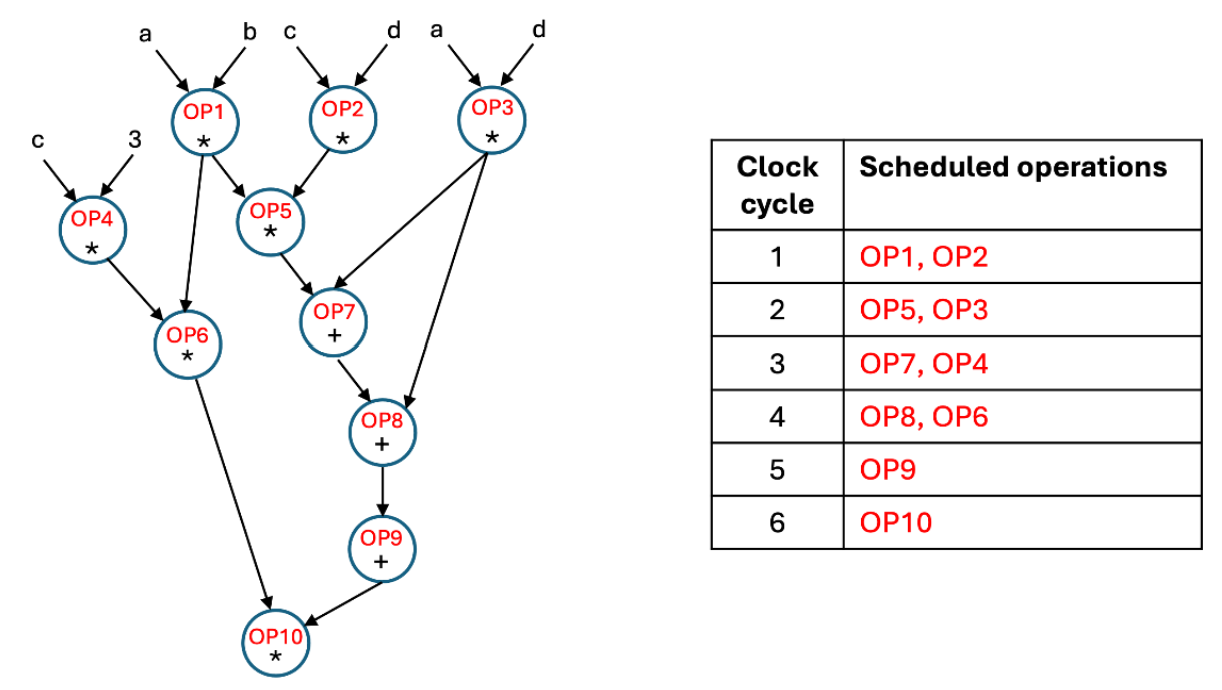
\includegraphics[width=0.7\textwidth]{images/dfg-hls.png}
\end{figure}

\begin{tcolorbox}
	The system is constrained by 2 multiplier, and at least 1 adder.
	We can tell because OP1, OP2, OP3, OP4 are all independent, yet they are not executed together (at most 2 multiplier operations
\end{tcolorbox}

\num How does the schedule from the previous question change if the available resources are 4 multipliers and 2 adders (all with 1 clock cycle latency)?

\begin{tcolorbox}
	\begin{center}
		\begin{tabular}{|c|l|l|}
			\hline
			\textbf{Clock Cycle} & \textbf{Scheduled Operations} \\ \hline
			1                    & OP1, OP2, OP3, OP4            \\ \hline
			2                    & OP5, OP6                      \\ \hline
			3                    & OP7                           \\ \hline
			4                    & OP8                           \\ \hline
			5                    & OP9                           \\ \hline
			6                    & OP10                          \\ \hline
		\end{tabular}
	\end{center}
\end{tcolorbox}

\num When is \texttt{cudaSetDevice()} used?

\begin{tcolorbox}
	\texttt{cudaSetDevice()} is used in multi-GPU environments to explicitly select which graphics card the current CPU thread should issue commands to.

	By default, a host thread operates on Device 0; if a system has multiple GPUs (e.g., Device 0 and Device 1), a developer must call cudaSetDevice(1) to switch the current thread's context to the second GPU before allocating memory or launching kernels on it.

	This setting is thread-local, meaning different CPU threads can simultaneously control different GPUs by calling this function with different device IDs.
\end{tcolorbox}

\num Describe the effect of the following OpenMP pragma:

\begin{minted}[autogobble]{text}
    #pragma omp target map(a,b)
\end{minted}

\begin{tcolorbox}
	This pragma instructs the compiler to offload the execution of the following code block to a target device (such as a GPU). The \texttt{map(a, b)} clause manages the data movement between the host (CPU) and the device: it allocates memory for variables \texttt{a} and \texttt{b} on the device, copies their values from Host to Device before the code executes, and copies the modified values back from Device to Host after the execution finishes.
\end{tcolorbox}

\num A Domain-Specific Language provides productivity and performance at the expense of generality. Is this statement true or false? Explain.

\begin{tcolorbox}
	\textbf{TRUE}.

	A Domain-Specific Language (DSL) explicitly sacrifices generalitynto optimize for a narrow purpose. By restricting the language's semantics, the compiler gains a deeper understanding of the code's intent, enabling it to perform aggressive domain-specific optimizations that maximize performance.

	Simultaneously, productivity improves because the language exposes high-level primitives that closely match the domain's model, allowing developers to describe what they want to compute rather than how to implement the low-level details.
\end{tcolorbox}

\num Describe the ASAP scheduling algorithm.

\begin{tcolorbox}
	The ASAP (As Soon As Possible) scheduling algorithm assigns every operation to the earliest possible clock cycle allowed by its data dependencies (assuming unlimited hardware resources).

	An operation is scheduled immediately after its latest predecessor has finished. While this guarantees the theoretical minimum possible total execution time (latency), it tends to creates a spike in resource usage at the beginning of the execution (often requiring more functional units than a real physical chip possesses).
\end{tcolorbox}

\num If we want to copy 3000 bytes of data from host array \texttt{h\_A} (\texttt{h\_A} is a pointer to element 0 of the source array) to device array \texttt{d\_A} (\texttt{d\_A} is a pointer to element 0 of the destination array), what would be an appropriate API call for this in CUDA?

\begin{tcolorbox}
	\begin{minted}[autogobble]{text}
        cudaMemcpy(d_A, h_A, 3000, cudaMemcpyHostToDevice);
    \end{minted}
\end{tcolorbox}

\num How is error handling implemented in a CUDA host program to check whether a kernel launch has been successful?

\begin{tcolorbox}
	Because kernels launch asynchronously and return \texttt{void}, the host program cannot directly check a return value for success. Instead, it must:

	\begin{enumerate}
		\item Call \texttt{cudagetLastError()} immediately after the kernel launch to catch synchronous error; followed by
		\item \texttt{cudaDeviceSynchronize()} to force the host to wait for the GPU to finish. This ensures that runtime errors are propagated back to the host, where they can be captured and translated into readable text using
		\item \texttt{cudaGetErrorString()}.
	\end{enumerate}
\end{tcolorbox}

\num What is asynchronous memory prefetching, and when is it useful?

\begin{tcolorbox}
	\textbf{Asynchronous memory prefetching} is a latency-hiding technique where data is fetched from slow global memory into the faster cache before the execution unit actually needs it, allowing the transfer to happen in parallel with current computations.

	It is useful in \textbf{bandwidth-bound} applications, such as matrix multiplication, where the processor would otherwise spend significant cycles stalled waiting for data to arrive.
\end{tcolorbox}

\num Why is synchronization necessary when programming with the shared memory model?

\begin{tcolorbox}
	Synchronization is necessary in the shared memory model to prevent \textbf{race conditions}, which occur when multiple threads attempt to access the same memory location simultaneously without a defined order.

	Without synchronization (like locks or barriers), the final result would depend from the unpredictable timing of thread execution.
\end{tcolorbox}

\num Sometimes a parallel program can be slower than a sequential one. Is this statement true or false? Why?

\begin{tcolorbox}
	\textbf{TRUE}.

	Parallelism always introduces \textbf{overhead}, such as the time required to create threads, synchronize them (locks/barriers), and communicate data between memory spaces. If the problem size is too small, the time spent managing these parallel tasks will be more than the time effectively saved by dividing the work.
\end{tcolorbox}

\num What is a DSL?

\begin{tcolorbox}
	A \textbf{DSL (Domain SPecific Language)} is a programming language specialized to a particular application domain. It has a restricted syntax making it more efficient at their specific purpose. There are two types of DSLs:
	\begin{itemize}
		\item \textbf{External}: a completely separate language (e.g., SQL, HTML, ...).
		\item \textbf{Embedded}: built on top of another language (like C++). It uses the host syntax but exploits its flexibility (e.g., pytorch on python). This is is easier to build (e.g., uses existing compilers) but it is constrained by the syntax rules of the host language.
	\end{itemize}
\end{tcolorbox}

\num For the \textbf{work-inefficient} scan kernel based on reduction trees, assume that we have 2048 elements in the input vector, explain how to estimate the number of add operations performed.

\begin{tcolorbox}
	In the \textbf{work-inefficient} scan, the algorithm makes $\log_2(N)$ iterative steps, (depth of the tree is $\log_2 N$). In each step, the algorithm performs a parallel addition ($\approx N$ steps). Therefore, the estimation for the total work is $O(N \log N)$ which for $N = 2048$, we have about $2048 \times \log_2 2048 = 2048 \log_2 11$ add operations.

	This is considered \textit{work-inefficient} because it performs significantly more operations than the theoretical minimum of $N - 1$ achieved by a sequential scan.
\end{tcolorbox}

\num For the \textbf{work-efficient} scan kernel based on reduction trees and inverse reduction trees, assume that we have 2048 elements in the input vector, explain how to estimate the number of add operations performed in both the forward and the reverse phase.

\begin{tcolorbox}
	In the \textbf{work-efficient} scan, the algorithm consists of two phases:

	\begin{enumerate}
		\item A reduction phase: the number of active elements halves at each step ($N/2 + N/4 + \dots + 1$), forming a geometric series that sums to $N - 1$ additions.
		\item An inverse reduction phase: traverses the tree in reverse to distribute sums, also performing $N - 1$ operations.
	\end{enumerate}

	Therefore, the estimation for the total work is $O(N)$, specifically $(N - 1) + (N - 1)$. For $N = 2048$, we perform $2047 + 2047 = 4094$ add operations.
\end{tcolorbox}

\num Describe the method to qualitatively evaluate a parallel algorithm through its data flow graph.

\begin{tcolorbox}
	To qualitatively evaluate a parallel algorithm using a Data Flow Graph, you analyze the structural geometry of the graph to determine two fundamental properties:
	\begin{itemize}
		\item Work ($T_1$): the total number of nodes in the graph, which represent the total volume of computation that must be performed;
		\item Critical path ($T_\infty$): the longest chain of dependent nodes from the start to the end of the graph.
	\end{itemize}

	The qualitative evaluation comes from comparing these two properties. A graph that is \textbf{wide and shallow} indicates high Average Parallelism ($T_1 / T_\infty$), meaning the algorithm scales well because many operations are independent.

	Conversely, a graph that is \textbf{narrow and deep} indicates a sequential bottleneck where the algorithm cannot run faster even with infinite processors.
\end{tcolorbox}

\num In Halide, it is better to start scheduling the input stage of the pipeline and proceed towards the output. Is this statement true or false? Explain.

\begin{tcolorbox}
	\textbf{FALSE}.

	In Halide, the scheduling strategy is typically consumer-driven, meaning you start with the output and work backwards to the inputs. You first define the loop structure for the final output stage, and then you schedule the producer stages (the intermediate steps or inputs) relative to that output.

	This approach ensures that values are computed and stored exactly when and where the consumer needs them, maximizing data locality and register reuse, which is difficult to achieve if you schedule inputs in isolation without knowing the consumer's access pattern.
\end{tcolorbox}

\num What are the characteristics of a program that make it amenable to parallelization with multiple threads?

\begin{tcolorbox}
	A program is amenable to parallelization if it exhibits a high degree of data independence, meaning its computational tasks or loop iterations can execute simultaneously without waiting for results from one another (no loop-carried dependencies). Also, the amount of computation per task should significantly outweighs the overhead of creating threads and synchronizing them.
\end{tcolorbox}

\num What are the characteristics of a program that make it amenable to parallelization on a GPU?

\begin{tcolorbox}
	A program is amenable to GPU parallelization if it exhibits \textbf{massive data parallelism}, meaning the same instruction sequence can be applied to multiple data elements simultaneously (SIMT). Unlike CPU threads, GPU threads require regularity: computations should have consistent control flow (minimal branch divergence) and memory access patterns should be coalesced (adjacent threads reading adjacent memory addresses).

	Additionally, the program should performing many calculations for every byte of data loaded from global memory, to effectively hide the latency of fetching data and keep the many cores utilized.
\end{tcolorbox}

\num Why would a programmer intentionally apply transformations that introduce redundant computation?

\begin{tcolorbox}
	To avoid the much higher cost of communication and memory access. In parallel systems, fetching a value from another processor or global memory (latency) is often much slower than simply re-calculating that value locally.
\end{tcolorbox}

\num Compare MPI, Pthreads, OpenMP, and CUDA according to how they describe parallelism and communication (i.e., implicitly/explicitly).

\begin{tcolorbox}
	\begin{itemize}
		\item \textbf{MPI}: handles parallelism and communication \textbf{explicitly}. You have to manage exactly how many processes run and you must explicitly send and receive data between processes.
		\item \textbf{Pthreads}: you explicitly manage every single thread using the API calls, but the communication is implicit (via shared memory).
		\item \textbf{OpenMP}: The parallelism is mostly implicit, you provide high-level directives (pragmas) and the compiler implicitly manages the threads. The communication is also implicis (via shared memory).
		\item \textbf{CUDA}: the parallelism is explicit, as you have to define the grid and block dimension (\texttt{<<<grid, block>>>}). The communication can be both explicit (there are API calls to transfer data between the host and the device) and implicit (threads communicate with each others in the same kernel via global memory).
	\end{itemize}
\end{tcolorbox}


\end{document}
